
\lecture{More Frequencies}{more-frequencies}
\section{More Frequencies}

\title{More Graphical Views of Frequency}
\subtitle{Section 2.2}

%\author{Kelly Black}
%\institute{Clarkson University}
\date{16 January 2012}

\begin{frame}
  \titlepage
\end{frame}

\begin{frame}
  \frametitle{Outline}
  \tableofcontents[hideothersubsections,sectionstyle=show/hide]
\end{frame}


\subsection{Clicker Question}


\begin{frame}
  \frametitle{Question:}

  Which plot below represents the Pareto chart for the following data:

    A, A, C, B, B, B, D

    \begin{tabular}{ccc}
      A: 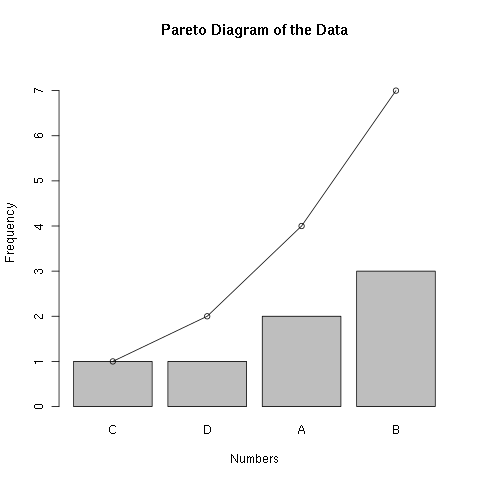
\includegraphics[width=3cm]{img/paretoQuizW1D2-a} &
      B: 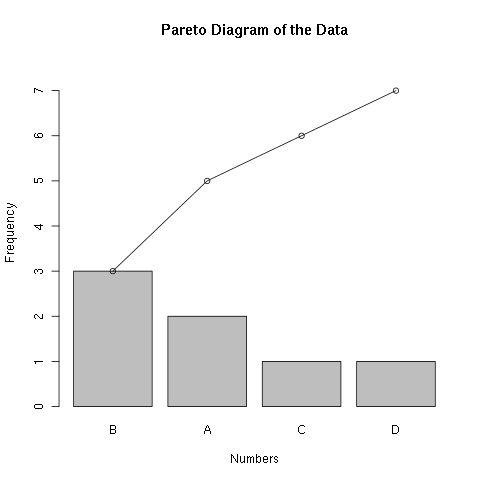
\includegraphics[width=3cm]{img/paretoQuizW1D2-b} &
      C: 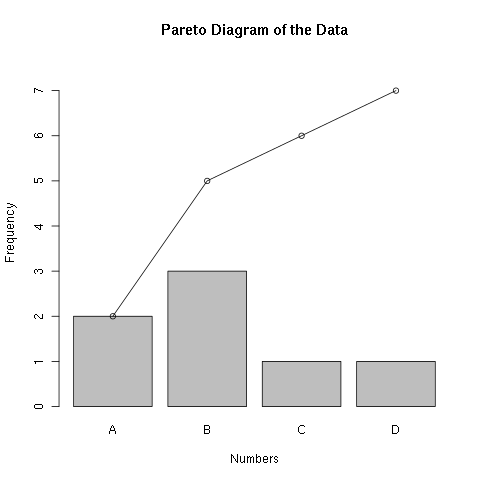
\includegraphics[width=3cm]{img/paretoQuizW1D2-c}
  \end{tabular}
  \uncover<2->{
    The answer is B
  }

\end{frame}


%\subsection{Frequency}
\subsection{Histograms}

\begin{frame}
  \frametitle{Histograms}

  Things to look for in a histogram:\\
  \begin{itemize}
  \item Spread
  \item Symmetry
  \item Evenness or variedness
  \item Skewness
  \item Mode
  \end{itemize}

\end{frame}


\begin{frame}
  \frametitle{Symmetry}

  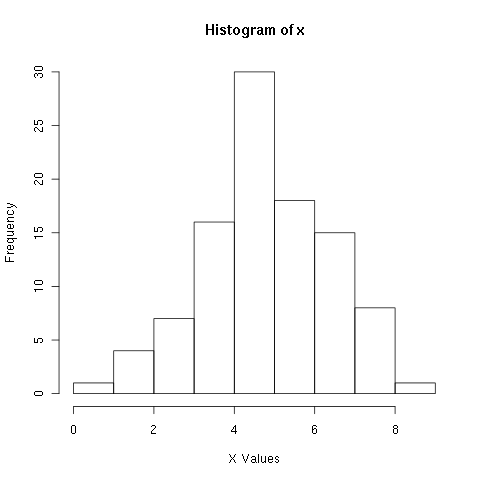
\includegraphics[width=7cm]{img/symmetricW1D2}

\end{frame}

\begin{frame}
  \frametitle{Uniformity}

  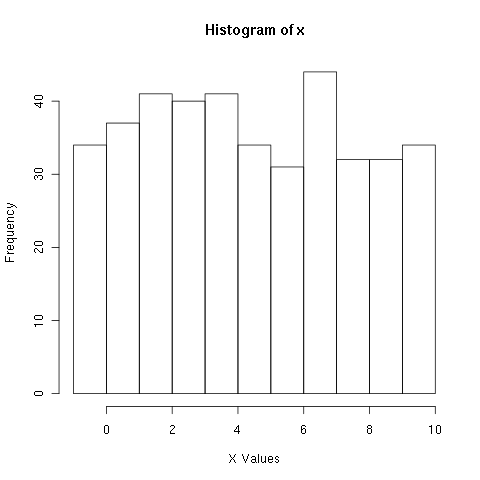
\includegraphics[width=7cm]{img/uniformW1D2}

\end{frame}


\begin{frame}
  \frametitle{Skewed Right}

  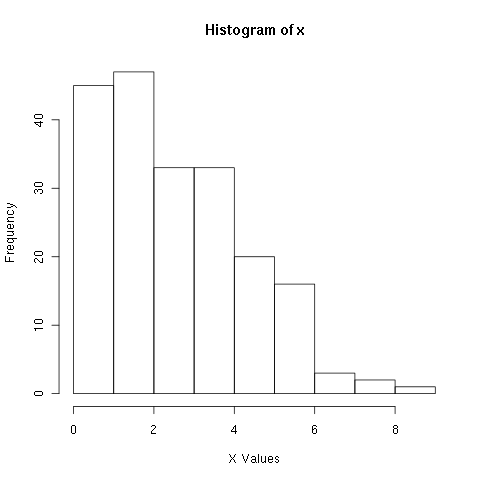
\includegraphics[width=7cm]{img/skewedRightW1D2}

\end{frame}


\begin{frame}
  \frametitle{Skewed Left}

  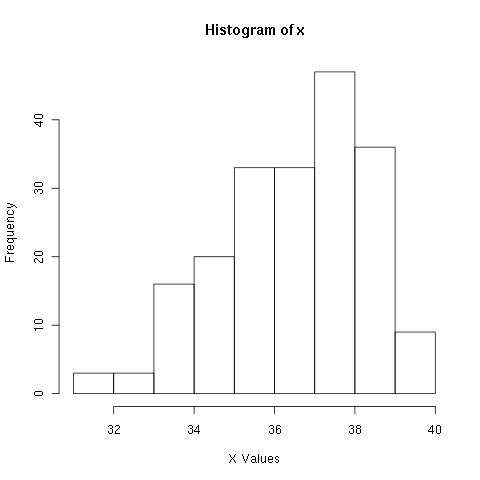
\includegraphics[width=7cm]{img/skewedLeftW1D2}

\end{frame}


\begin{frame}
  \frametitle{Bimodal}

  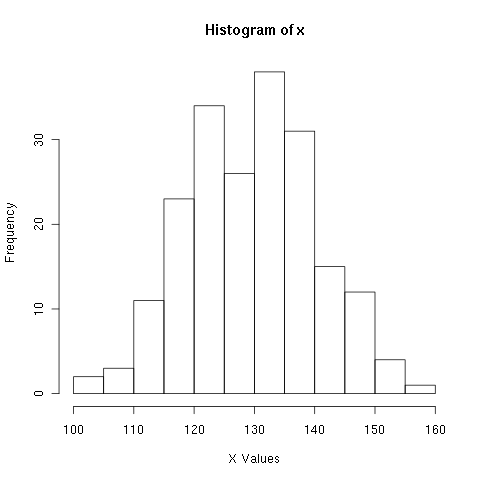
\includegraphics[width=7cm]{img/bimodalW1D2}

\end{frame}


\subsection{Cumulative Frequency}


\begin{frame}
  \frametitle{Cumulative Frequency}

  \begin{definition}
    The Cumulative Frequency is the frequncy of occurances for each
    result \textbf{less} than the given value.
  \end{definition}

\end{frame}


% LocalWords:  Clarkson pausesection hideallsubsections ccc
